\documentclass{standalone}

\usepackage{tikz}
\usepackage{standalone}
\usetikzlibrary{calc}

\begin{document}
    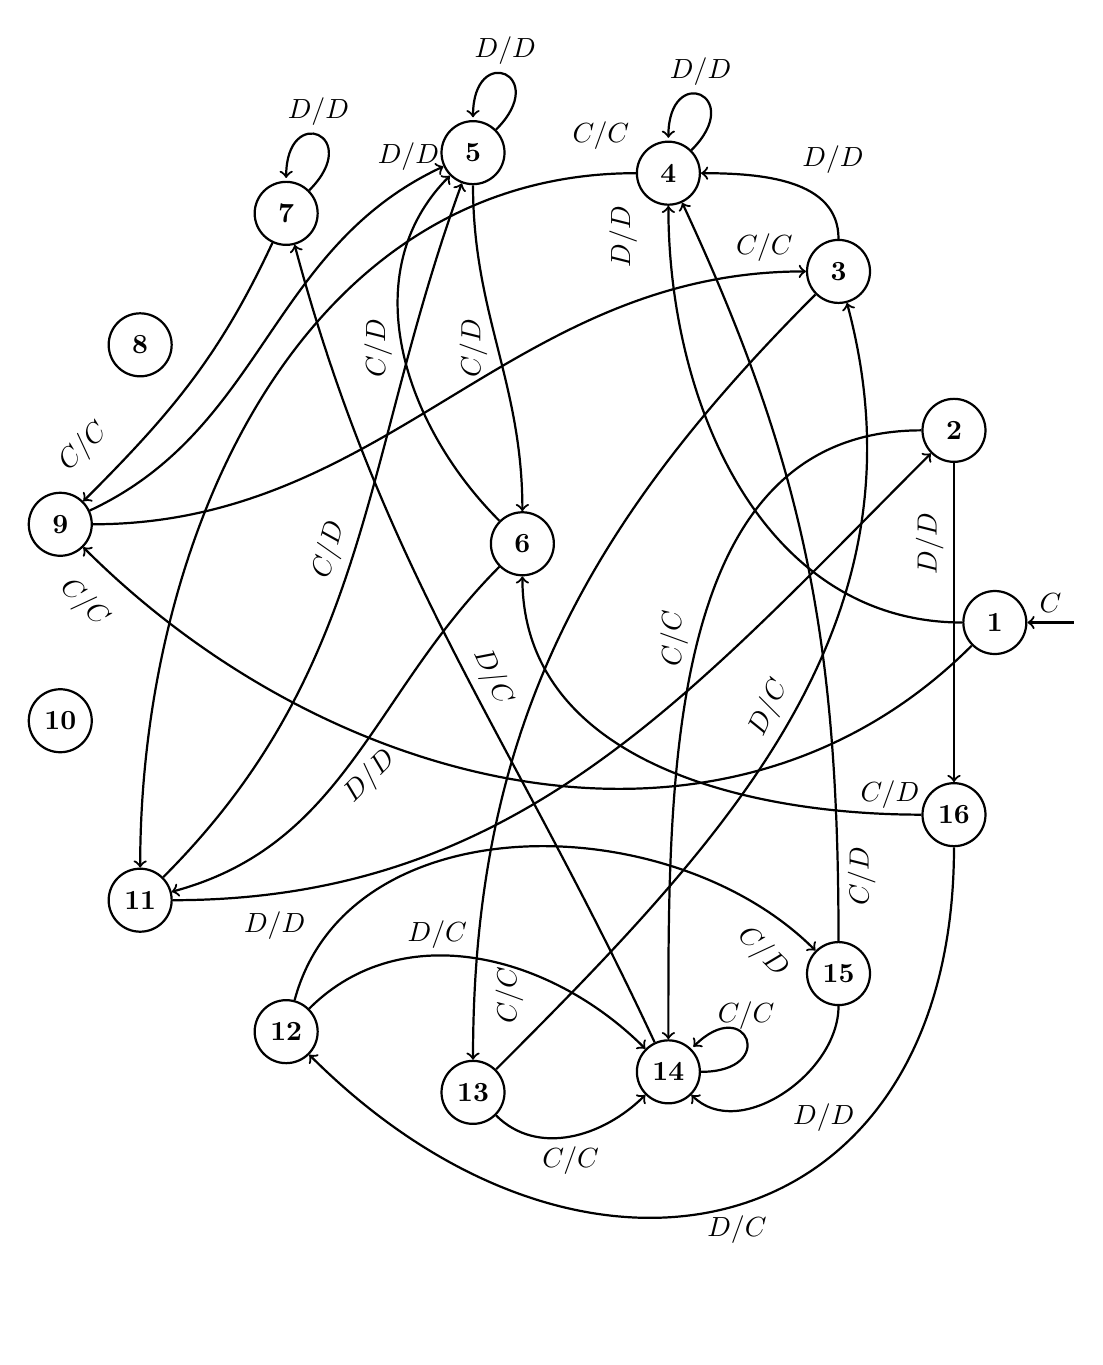
\begin{tikzpicture}

    \tikzstyle{state}=[minimum width=0.8cm, font=\boldmath];


    \node[circle, draw=black, thick] (0) at (0.0: 6cm) [state]    {$1$};
    \node[circle, draw=black, thick] (1) at (24.0: 6cm) [state]   {$2$};
    \node[circle, draw=black, thick] (2) at (48.0: 6cm) [state]   {$3$};
    \node[circle, draw=black, thick] (3) at (72.0: 6cm) [state]   {$4$};
    \node[circle, draw=black, thick] (4) at (96.0: 6cm) [state]   {$5$};
    \node[circle, draw=black, thick] (6) at (120.0: 6cm) [state]  {$7$};
    \node[circle, draw=black, thick] (7) at (144.0: 6cm) [state]  {$8$};
    \node[circle, draw=black, thick] (8) at (168.0: 6cm) [state]  {$9$};
    \node[circle, draw=black, thick] (9) at (192.0: 6cm) [state]  {$10$};
    \node[circle, draw=black, thick] (10) at (216.0: 6cm) [state] {$11$};
    \node[circle, draw=black, thick] (11) at (240.0: 6cm) [state] {$12$};
    \node[circle, draw=black, thick] (12) at (264.0: 6cm) [state] {$13$};
    \node[circle, draw=black, thick] (13) at (288.0: 6cm) [state] {$14$};
    \node[circle, draw=black, thick] (14) at (312.0: 6cm) [state] {$15$};
    \node[circle, draw=black, thick] (15) at (336.0: 6cm) [state] {$16$};

    \node[circle, draw=black, thick] (5) at (0, 1) [state]   {$6$};

    \coordinate[right of=0] (s);

    \draw (s) edge[out=180, in=0, ->, thick] node [above] {$C$} (0);

	\draw (0) edge[out=-135, in=-45, ->, thick] node [above left, xshift=-5.5cm, yshift=1.7cm, rotate=-45] {$C/C$} (8);
	\draw (0) edge[out=180, in=-90, ->, thick] node [below, xshift=-1.8cm,yshift=3.2cm, rotate=90] {$D/D$} (3);

    \draw (1) edge[out=180, in=90, ->, thick] node [above, rotate=90] {$C/C$} (13);     
    \draw (1) edge[out=-90, in=90, ->, thick] node [above, yshift=1cm, rotate=90] {$D/D$} (15);     

    \draw (2) edge[out=-135, in=90, ->, thick] node [above, rotate=90, xshift=-4.5cm, yshift=0.3cm] {$C/C$} (12);     
    \draw (2) edge[out=90, in=0, ->, thick] node [above right] {$D/D$} (3);   

    \draw (3) edge[out=180, in=90, ->, thick] node [above right, xshift=3.8cm, yshift=3cm] {$C/C$} (10);     
    \draw (3) edge[out=45, in=90, ->, thick, loop] node [above] {$D/D$} (3);  

    \draw (4) edge[out=-90, in=90, ->, thick] node [above, rotate=90] {$C/D$} (5);      
    \draw (4) edge[out=45, in=90, ->, thick, loop] node [above] {$D/D$} (4); 

    \draw (5) edge[out=135, in=-135, ->, thick] node [above, rotate=90] {$C/D$} (4);      
    \draw (5) edge[out=-135, in=15, ->, thick] node [below, rotate=45] {$D/D$} (10); 

    \draw (6) edge[out=-115, in=45, ->, thick] node [above left, xshift=-0.8cm, yshift=-0.7cm, rotate=45] {$C/C$} (8);      
    \draw (6) edge[out=45, in=90, ->, thick, loop] node [above] {$D/D$} (6); 

    \draw (8) edge[out=0, in=180, ->, thick] node [above, xshift=4cm, yshift=1.6cm] {$C/C$} (2);      
    \draw (8) edge[out=25, in=-155, ->, thick] node [above, xshift=1.8cm, yshift=2cm] {$D/D$} (4);  

    \draw (10) edge[out=45, in=-110, ->, thick] node [above, rotate=75] {$C/D$} (4);     
    \draw (10) edge[out=0, in=-135, ->, thick] node [below, xshift=-4cm, yshift=-1.7cm] {$D/D$} (1);  

    \draw (11) edge[out=75, in=135, ->, thick] node [above right, xshift=2.5cm, yshift=-1.2cm, rotate=-45] {$C/D$} (14);    
    \draw (11) edge[out=45, in=135, ->, thick] node [above left] {$D/C$} (13);    

    \draw (12) edge[out=-45, in=-135, ->, thick] node [below] {$C/C$} (13);    
    \draw (12) edge[out=45, in=-75, ->, thick] node [above, rotate=65] {$D/C$} (2);

    \draw (13) edge[out=0, in=45, ->, thick, loop] node [above] {$C/C$} (13);    
    \draw (13) edge[out=115, in=-75, ->, thick] node [above right, rotate= -65] {$D/C$} (6);  

    \draw (14) edge[out=90, in=-65, ->, thick] node [above, yshift=-4cm, xshift=1cm, rotate=90] {$C/D$} (3);     
    \draw (14) edge[out=-90, in=-45, ->, thick] node [below right] {$D/D$} (13);  

    \draw (15) edge[out=180, in=-90, ->, thick] node [above, xshift=3cm, yshift=-0.7cm] {$C/D$} (5);     
    \draw (15) edge[out=-90, in=-45, ->, thick, looseness=1.5] node [below] {$D/C$} (11);    
    \end{tikzpicture}
\end{document}